%\usepackage{geometry}

%\usepackage{graphicx}
%\usepackage{color,framed}
%\usepackage[print,1to1]{booklet} %print option switches to landscape
%\pagespersignature{16}
%\setpdftargetpages
\documentclass[letterpaper,12pt]{memoir}
\newsavebox{\FrontImgBox}
\newlength{\FrontClip}

\usepackage[pdftex]{graphicx}
%block size info
\settypeblocksize{7.25in}{4.5in}{*}
\addtolength{\textheight}{\onelineskip}
\setlrmargins{2.1in}{*}{1}
\setulmargins{1.75in}{*}{1}
\checkandfixthelayout
\usepackage{todonotes}
\pagestyle{empty} % no page number
\usepackage[pdftex]{graphicx}
\usepackage{eso-pic}

\settypeblocksize{7.25in}{4.5in}{*}
\addtolength{\textheight}{\onelineskip}
\setlrmargins{2.1in}{*}{1}
\setulmargins{1.75in}{*}{1}
\checkandfixthelayout
 \usepackage{microtype} % better justification & protrusion
\usepackage{newtxtext} % Times-like body text (newspaper vibe)
\usepackage[scaled]{helvet} % Sans for headlines and decks
\usepackage[T1]{fontenc}
\usepackage[utf8]{inputenc}

% ====== Columns & visuals ======
\usepackage{multicol}
\setlength{\columnsep}{0.28in}
\setlength{\columnseprule}{0.2pt}

\usepackage{graphicx}
\usepackage{wrapfig}
\usepackage{caption}
\captionsetup{font=small,labelfont=bf}

\usepackage[dvipsnames]{xcolor}
\usepackage{lettrine} % drop caps
\usepackage[many]{tcolorbox} % pull quotes / sidebars
\usepackage[print,1to1]{booklet} %print option switches to landscape
\pagespersignature{16}

\tcbset{
  colback=black!2,
  colframe=black!40,
  boxsep=4pt, left=6pt, right=6pt, top=6pt, bottom=6pt,
  sharp corners,
}

% ====== Headings & bylines ======
\setsecheadstyle{\Large\bfseries\sffamily}
\setsubsecheadstyle{\normalsize\bfseries\sffamily}
\setsubsubsecheadstyle{\normalsize\itshape}

\newcommand{\kicker}[1]{\textsf{\bfseries\small\color{Gray} #1}}
\newcommand{\headline}[1]{\textsf{\bfseries\fontsize{34}{36}\selectfont #1}}
\newcommand{\deck}[1]{\textsf{\large\itshape #1}}
\newcommand{\byline}[1]{\textsf{\small\color{Gray} Af #1}}
\usepackage{tikz}
\usetikzlibrary{fadings,patterns}

% Define a generic "fade to transparent" around a rectangle
\tikzfading[name=image fade,
  inner color=transparent!50,
  outer color=transparent!100]

  % Text outline ("border around letters")
\usepackage{contour} % works with pdfLaTeX/XeLaTeX/LuaLaTeX
\contourlength{0.9pt}         % default stroke thickness
\contournumber{32}            % smoothness of the outline

% Helpers: white text with dark outline (and a thinner variant)
\newcommand{\ow}[2][black]{\contour{#1}{\textcolor{white}{#2}}}
\newcommand{\owthin}[2][black]{%
  \begingroup\contourlength{0.6pt}\contour{#1}{\textcolor{white}{#2}}\endgroup}

% ====== Page banner / folio ======
\makepagestyle{newspaper}
\makeoddhead{newspaper}{\textsf{\small Den Rullende Sten}}{}{\textsf{\small Sponsoreret af Det Glemte Akademi}}
\makeevenhead{newspaper}{\textsf{\small Sponsoreret af Det Glemte Akademi}}{}{\textsf{\small Den Rullende Sten}}
\makeoddfoot{newspaper}{}{\textsf{\small\thepage}}{}
\makeevenfoot{newspaper}{}{\textsf{\small\thepage}}{}
\makeheadrule{newspaper}{\textwidth}{0.4pt}
\pagestyle{newspaper}

% ====== Pull quote and sidebar environments ======
\newenvironment{pullquote}
  {\begin{tcolorbox}\itshape\large}
  {\end{tcolorbox}}


\usepackage{xparse}
\usepackage{wrapfig}

% Justérbare standarder for sidebar i spalter
\newcounter{sidebarlines}              % hvor mange linjer der skal "wrappe" forbi boksen
\setcounter{sidebarlines}{14}
\setlength{\sidebarwidth}{0.42\columnwidth}


% ====== Utilities ======
\newcommand{\separator}{%
  \par\noindent{\color{black!40}\rule{\textwidth}{0.4pt}}\par
}


% Front feature image: spans \textwidth, keeps aspect ratio, fades at edges,
% and overlays outlined text (no boxes).
% Usage: \FrontFeatureImage{<image>}{<kicker>}{<headline>}{<deck>}{<credit>}
\newcommand{\FrontFeatureImage}[5]{%
  % Typeset image at \textwidth just once and measure its height
  \sbox{\FrontImgBox}{\includegraphics[width=\textwidth]{#1}}%
  % Total height of the scaled image (height + depth)
  \dimen0=\dimexpr\ht\FrontImgBox+\dp\FrontImgBox\relax
  % Max allowed height
  \dimen2=.75\textheight
  % Choose visible height: min(actual, max)
  \ifdim\dimen0>\dimen2
    \setlength{\FrontClip}{\dimen2}%
  \else
    \setlength{\FrontClip}{\dimen0}%
  \fi
  %
  \begin{tikzpicture}
    % Define a "frame" we’ll use for anchors & clipping
    \coordinate (TL) at (0,0);                       % top-left
    \coordinate (TR) at (\textwidth,0);              % top-right
    \coordinate (BL) at (0,-\FrontClip);             % bottom-left (cropped)
    \coordinate (BR) at (\textwidth,-\FrontClip);    % bottom-right (cropped)

    % Image with soft fading edges, clipped to the frame (crops from the bottom)
    \begin{scope}
      \clip (TL) rectangle (BR);
      \node[anchor=north west, inner sep=0pt,
            path fading=image fade, fit fading=false] at (TL)
        {\usebox{\FrontImgBox}};
    \end{scope}

    % Dark wash for legibility, also softly faded (match the same clip)
    \begin{scope}
      \clip (TL) rectangle (BR);
      \fill[black,opacity=0.30, path fading=image fade] (BL) rectangle (TR);
    \end{scope}

    % Text stack (bottom-left) — outline style preserved
    \node[anchor=south west, xshift=1em, yshift=1em, align=left,
          text width=.75\textwidth] at (BL){%
      \sffamily
      % Kicker (optional)
      \if\relax\detokenize{#2}\relax\else
        {\owthin[black!85]{\textsf{\bfseries\small #2}}}\\[0.15em]\fi
      % Headline
      {\ow{\bfseries
        \resizebox{1\textwidth}{!}{#3}%
      }}\\[0.2em]
      % Deck
      {\owthin{\large\itshape #4}}%
    };

    % Credit (bottom-right), small outline
    \node[anchor=south east, xshift=-1em, yshift=1em] at (BR)
      {\sffamily\small \owthin[black!85]{#5}};
  \end{tikzpicture}%
}





\begin{document}
\pdfpageheight=\paperwidth
\pdfpagewidth=\paperheight
\paperwidth=\pdfpagewidth
\paperheight=\pdfpageheight 
% ====== Nameplate ======
\begin{figure}
  \begin{center}
      
\includegraphics[width=0.98\textwidth]{Logo.png}%
  \end{center}    
\end{figure}
\begin{center}
  {\Large\sffamily Udgave 126}
\end{center}


% Front feature image (keeps aspect ratio, spans \textwidth)
\FrontFeatureImage{Dæmon.png}
{EKSKLUSIVT}
{Blodets Broderskab I Nordland!}
{"Godt klaret" udtaler dæmonerne}
{}

\vspace{.75\baselineskip}


% ====== Lead story (Front page) ======
\par\medskip
\headline{Blodets Broderskab opkøber land}
\par\medskip
\deck{Mange siger at indflydelsen fra Blodets Broderskab spreder sig, men Imperiet mener ikke der er noget at bekymre sig om.}
\par\medskip
\byline{Kirsten Giftkniv}
\medskip

\lettrine[lines=3,lhang=0.1,loversize=0.05]{B}{lodets} Broderskab er en relativt ukendt organisation. De udfordre den mono-normative opsætning som Imperiet spreder, hvor der udstilles krav at man ikke skal lave aftaler med dæmoner. Blodets Broderskab fremstiller en anden vej. En model hvor dæmonerne kan forhandles med. De forslår fred i en verden af kaos.

\begin{pullquote}
“Efter dæmonkrigen har dæmonerne fået et dårligt ry. Vi mener at en fredelig løsning kan udarbejdes, og vi er på nuværende tidspunkt i samtaler med dem for at opnå en dialog om en forenet velfærds stat som kan sætte fokus på de kerne værdier som alle medlemmer af Imperiet jo støtter op om.”\\
\textit{- Udtaler Thorleif Bør'nemorder, Talsmand for Blodets Broderskab}
\end{pullquote}

Vi har ragt ud til Imperiet for kommentar, men har fået at vide at Imperiets indflydelse står stærkt og dette agressive indkøb i Permersland og Nordland ikke vil ændre på nuværende lokal politik. Det er dog åbenlyst at pengene til disse indryk kommer fra et andet sted, og efter at have lavet en smule efterforskning så er det tydeligt at magter udenfor Imperiet sender store mængder af Fjend til Blodets Broderskab. 

Gennem effektiv journalistik er vi ved Den Rullende Sten kommet frem til at disse midler kommer fra A'kastin. Da vi forsøgte at række ud til deres ny-udnævnte konge, så for vores journalist vild, og fik i stedet kontakt til nogle lokale dæmoner.

\begin{pullquote}
“Godt klaret! Vi har altid set Blodets Broderskab som en allieret i kampen mod had og kaos.”\\
\textit{- Udtaler Yultraf, udvalgt af Hadets Ærkedæmon og Kaosets Ærkedæmon}
\end{pullquote}

Hvis nogen finder resterne af vores udsendte praktikant til A'kastin, så kan deres udstyr sendes til Det Glemte Akademi.

\subsection*{Sjæleindekset}
Vi har naturligvis via vores netværk fået førsteklasses insiderinfo om de varmeste sjæle på markedet lige nu! For at hjælpe dig med at træffe informerede beslutninger, har vi udviklet Sjæleindekset™, der viser hvilke sjæle der er i vækst, og hvilke der allerede er pantsat til overpris. Med andre ord: du kan nu sammensætte en sjælportefølje, der ikke alene imponerer selv den mest kyniske dæmon, men også vil hjælpe dig med at finde den rigtige sjæl at investere i.

Fornyligt har vi set opkøb af følgende sjæle fra magtfulde dæmoner! Kom ind på stue-etagen og invester før de bliver populære!\\
\begin{table}[htbp]
\begin{tabular}{l|r}
Person & Stigning \\ \hline
Asker Grønfjer & Op 2 Tjenester\\
Bob &  Op 1 Tjeneste \\
Boran & Op 1 Tjeneste  \\
Dorian Vinterkrone &  Op 1 Tjeneste \\
Lerik &  Op 1 Tjeneste \\
Noriel &  Op 1 Tjeneste \\
Robin &  Op 1 Tjeneste \\
Thorgaard &  Op 1 Tjeneste \\
Vilhelm Nydelhosen &  Op 1 Tjeneste 
\end{tabular}
\end{table}

\subsection*{Nyheder}
\subsubsection*{Drage bryder løs i Salezstad}
Som vi skrev om i sidste måned, blev der fornyligt født et nyt drageæg i fangeskab. Dette drageæg lader til at være lidt af en udbryderkonge. Natten til Onsdag brød drageægget nemlig ud af sit bur, hvorefter det flygtede ud gennem hovedstadens gader, fortæller Vagtkaptajn Hammer. 

\begin{pullquote}
“Det er den eneste logiske forklaring på hvordan det er kommet ud af sit bur, til borgmesterens kontor, uden nogen af dyrepasserne har set noget.”\\
\textit{- Udtaler Vagtkaptajn Hammer.}
\end{pullquote}

Esselaia kirken har erklæret det er mirakel at ægget allerede har kunnet bevæge sig, og forlanger at det bliver overleveret til deres varetægt. Den Royale Zoo har sagt at Esselaia's kult ingen indflydelse har ved dem og de vil derfor ikke overlevere ægget.

\subsubsection*{Nye runer solgt!}
Sidste måned opdagede Hammerens Krak 3 nye typer af runer. Disse blev sendt til A'kastin for at undgå en potentiel udryddelse af Livets Ende når runerne blev testet. Øksens Krak kan nu raportere at disse runer er blevet solgt til højest bydende, hvilket har vagt dyb vrede ved beboerne af Livets Ende.

\begin{pullquote}
“Aldrig har jeg i mine dage set så respektløs opførsel. [...] Og vi har derfor valgt at dræbe 500 Sortelvere.”\\
\textit{-Udtaler Than Ülwrick Krezz}
\end{pullquote}

Bekymring om at medlemmer af Blodets Broderskab skulle få adgang til disse runer betyder at Livets Ende har taget kontakt til Imperiet for at stoppe Blodets Broderskab og deres indflydelse i Nordland samt Permersland.

\subsubsection*{Religion: Morwen udgiver nye love til følgere}
Morwen er den nyeste gud til Kalish. Som mange tilbedere har kunnet fornæmme er denne religion kædet sammen med korruption og dæmon handler. Dette skyldes blandt andet Morwens fortid som tidligere Ærkedæmon. For at gøre op for dette har gudinden for Død, Handel og Tid samlet sine følgere, og de har lavet 13 nye bud som skal følges af alle Morwen tilbedere.
\begin{enumerate}
\item Stræb altid efter en balance mellem synder og dyder.  
\item Bevar sjælens helhed, som den blev skænket dig.  
\item Al udøvelse af nekromanti er forbudt og skal forkastes.  
\item Al handel skal ske i retfærdighed blandt de troende.  
\item Fremsig daglig bøn for Den Højhellige Morwen.  
\item Yd kirkeskatten efter evne og oprigtighed.  
\item Vis dine medtroende broderlig respekt.  
\item Sæt din lid til præstens ord, som er givet af Morwen.  
\item Værn om både livet og døden, thi begge er hellige.  
\item Løft ej våben mod andre end de vantro.  
\item Overvej dine handlinger med from alvor og visdom.  
\item Tag ikke imod handel, der er uretfærdig eller besmittet.  
\item Hvil dig på Morwens dag, søndag.  
\end{enumerate}

\subsubsection*{Dæmoner vandre gennem A'kastin og laver aftaler}
Kelllwan kirken har bekræftet at rygterne om syv dæmoner der har vandret gennem A'kastin fra Leltho er korrekt. De fortæller at især en af dæmonerne havde lavet utrolig mange aftaler med dødelige, og havde derfor mere magt end forventet. Dette medførte at Kelllwan's Messias måtte træde tilbage fra forhandlingerne i Permersland for at udrydde disse dæmoner personligt. Kelllwan kirken fortæller at alle disse dæmoner, med undtagelse af en, er blevet udryddet.\\
Dæmonen der undslap siges at være utrolig stærk da den havde indgået en aftale med blandt andet den nye Konge af Akastin. Imperiet benægter at det skulle være gennem en sådan aftale at den nye konge er kommet til magten, men vi har ikke hørt noget fra kongen selv.\footnote{Vi har heller ikke spurgt.}

\subsubsection*{Den stærkeste kriger i A'kastin fundet!}
Den nye konge af A'kastin har valgt at holde en turnering for at finde den stærkeste kriger i hele A'kastin. Under denne turnering var der flere problemer med sortelvere, og vidner mener at de også har set flere Orkere og Gobliner deltage i turnering. Det viste sig dog at være et menneske i byen Marcustad, som vandt turnering. Den Kejserlige Livsvagt har valgt at give et tilbud om træning og praktik plads til vinderen af turnering. De Hvide Fjer har ikke givet det samme tilbud, da de ikke mener at en kamp hvor orkere kan deltage er værdig nok til at kunne få plads blandt deres rang.

\subsubsection*{Kaos træ i problemer}
En ærkedruide fra Mek udtaler at de har observeret problemer med kaos træet. Dette kunne påvirke verden træet. 

\begin{pullquote}
“Vi har observeret verdenstræet hælder mod syd-øst. Dette indikere at kaos træet er i fare. Det er derfor vigtigt at finde en Kelllwan, Esselaia eller Morwen Præst og få dem til at velsigne et stykke Cedertræ og begrave det i den lokale urtedal. Dette vil sikre kaos træets stabilitet.”\\
\textit{-Udtaler Ærkedruide Pjuskebusk}
\end{pullquote}

\subsubsection*{Dronningens Fornærmede Stolthed: Et Angreb på Marcusstad}
\byline{Marcudsstadts Råd for Fred og Retfærdighed}\\
Da Kong Dorian Vinterkrone indførte den retfærdige lov om, at ingen fremmede måtte bære trukne våben i Marcusstad, svarede sortelverdronningen, Niel, ikke med fornuft, men med fornærmelse og hovmod. Hendes stolthed kunne ikke bære, at orden og lov gik forud for hendes folk og deres barbariske skikke.\\
\begin{wrapfigure}[20]{r}{0.52\textwidth}
  \vspace{-6pt}
  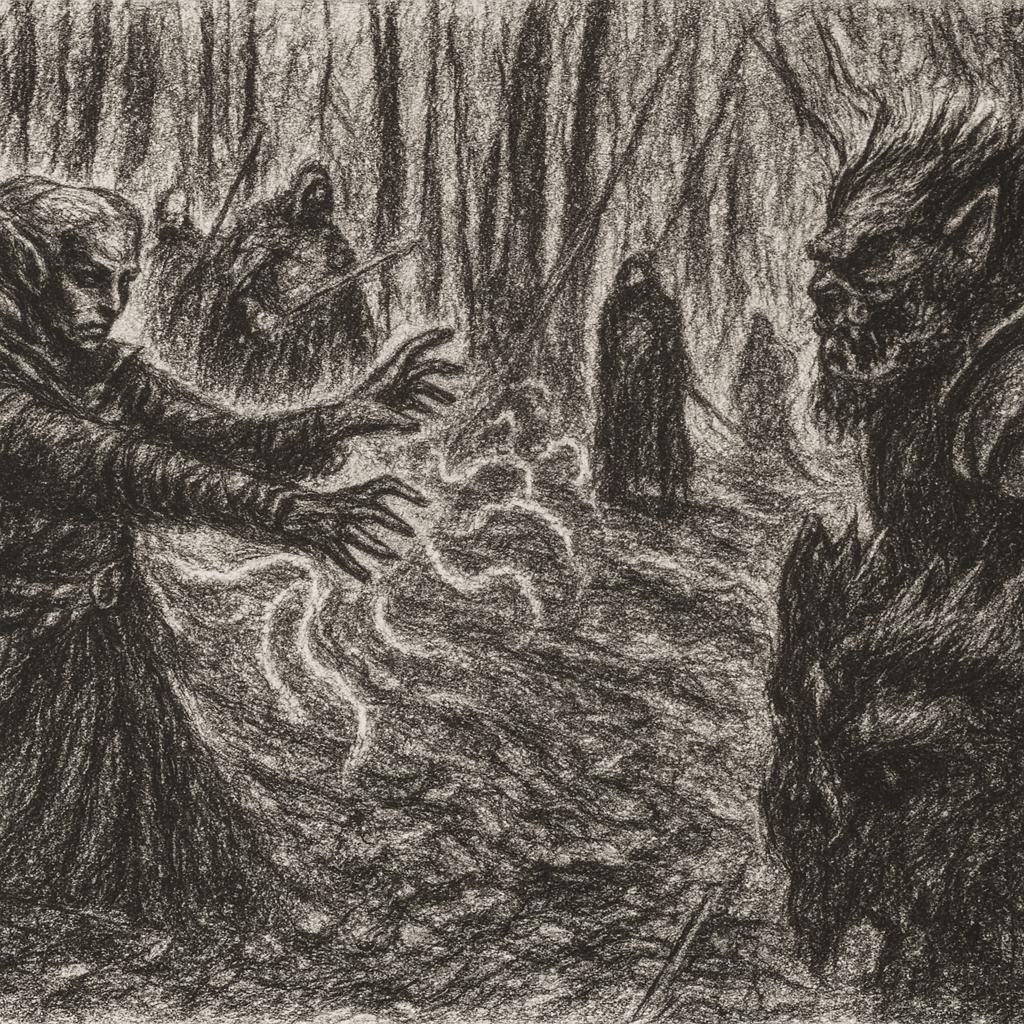
\includegraphics[width=0.52\textwidth]{Smædebillede.png}
  \caption*{\sffamily\small Sortelverdronning Niel angriber de selvsamme orkere som hun har indgået alliance med. Eksperter spørger: "Er der nongen hun ikke vil stikke i ryggen?"}
  \vspace{-6pt}
\end{wrapfigure}
Drevet af vrede forenede hun sig med de brutale orker og beordrede et angreb mod vores by. Men under kongens urokkelige lederskab blev forsøget knust. Vore mure, vores soldater og ikke mindst Dorians retfærdige hånd viste, at Marcusstad ikke lader sig true af mørkets dronning.\\

Hvor hun vælger krig og kaos, står Kong Dorian som folkets beskytter, et fyrtårn af fred, lov og orden. Hans visdom og styrke samler os, og under hans krone vil Marcusstad altid forblive stærk.\\

\begin{pullquote}
“Sikke dog en barnlig opførsel”\\
\textit{- Udtaler en tilfældig person fundet på gaden}
\end{pullquote}

{\tiny Denne artikel var sponsoreret af Kong Dorian Vinterkrone}

\newpage
\par\medskip
\headline{Tema: Hvem er Inkvisitionen?}
\par\medskip
\deck{Vi tager hul på den mystiske orden, der lever i skyggerne. I dette eksklusive interview går vi et spadestik dybere.}
\par\medskip
\byline{Stefani Ervind}
\medskip

\lettrine[lines=3,lhang=0.1,loversize=0.05]{Æ}{rede} læsere. Jeg har før bragt jer temaerne som i alle elsker: "Esselaia: Gud eller Kult?" og "Hvorfor holder de ikke bare fred i Permersland?". Jeg har denne gang fået et eksklusivt interview med et tidligere medlem af Inkvisitionen. Erik Frosch, taler ud om sine oplevelser, og igennem de næste mange uger vil vi tage hul på hvem Inkvisitionen er og hvordan de blev stiftet.\\
\begin{wrapfigure}{r}{0.52\columnwidth}
  \vspace{-6pt}
  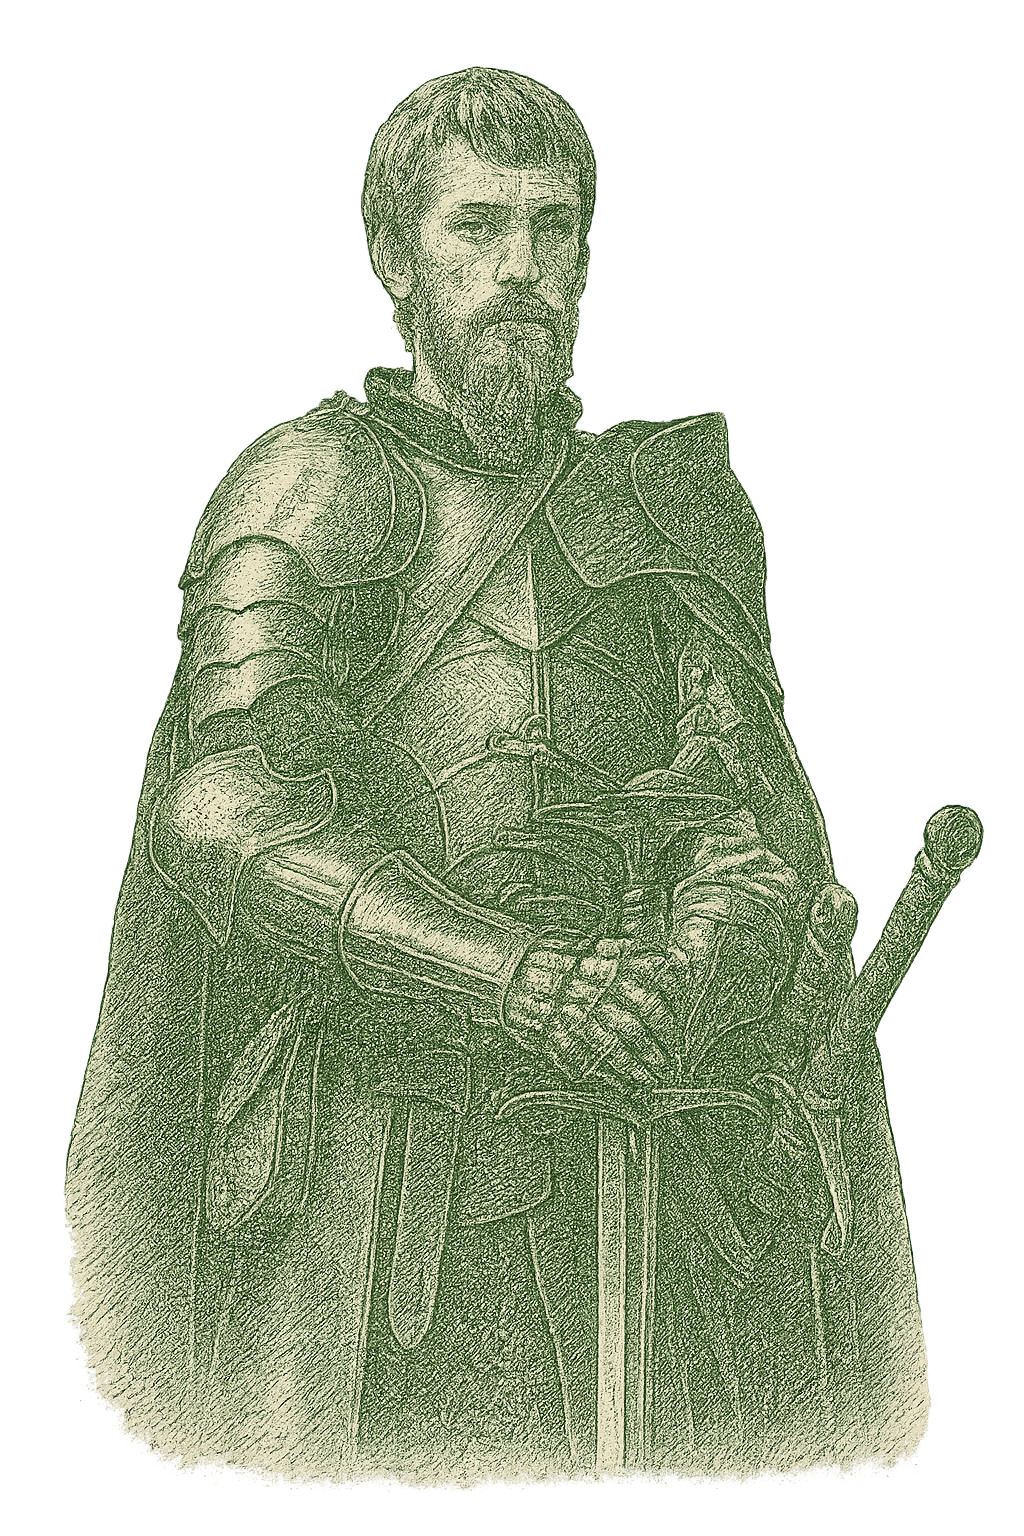
\includegraphics[width=0.52\columnwidth]{Martin.png}
  \caption*{\sffamily\small Det eneste billede vi har af en inkvisitør i vores arkiv. Inkvisitør Arno.}
  \vspace{-6pt}
\end{wrapfigure}

\textbf{Stefani:} Agent Frosch, kan De beskrive Inkvisitionens arbejde for vores læsere?\\
\textbf{E. Frosch:} Naturligvis. Vores opgave er at beskytte folket mod dæmoner, hekseri og mistænkelige hendelser. Jeg har selv været en del af den 3. Orden. Dette var kendt som Skjoldets Orden.\\

\textbf{Stefani:} Spændende. Hvad er Deres mest mindeværdige sag?\\
\textbf{E. Frosch:} Det må være i landsbyen Brondal, just nord for grænsen til isgletjserne. Køerne holdt op med at give mælk. Vi antog straks dæmonologisk aktivitet, muligvis knyttet til den lokale præst. Som regel er det den lokale præst der står bag den slags, så vi torturere dem for en sikkerheds skyld.\\

\textbf{Stefani:} Og hvad gjorde De ved denne mangel på mælk?\\
\textbf{E. Frosch:} Efter det blev klart at det ikke var præsten, så betalte vi naturligvis for hans begravelse, og vi satte hele byen i karantæne. Vores hold forhørte alle, og til sidst konkluderede vi, at en enke bagte brød, der var alt for godt. Vi brændte hendes ovn, hendes hus og… ja, flere nabo huse også. Ganske enkelt for at sørge for at intent dæmonisk skulle overleve.\\

\textbf{Stefani:} Gav det resultat?\\
\textbf{E. Frosch:} Dagen efter gav køerne mælk igen. Så vi erklærede missionen for en succes. Først senere fandt vi ud af, at malkepigen bare havde været på ferie. Men ikke desto mindre fandt vi ud af folket var villige medlemmer af Imperiet.\\

\textbf{Stefani:} Fortryder De ikke den beslutning?\\
\textbf{E. Frosch:} Absolut ikke. Som Højinkvisitør Stjernefødt siger: Når sværd smedes, vil de bære eller bryde. Og i Brondal brød de. Så vi bar dem til bålet.\\

Det er tydeligt for mig, kære læsere, at der er flere folk i Inkvisitionen som misbruger denne magt som de har. Jeg stiller dem derfor dette spørgsmål. Er den ubestridte magt de får givet nødvendig for at beskytte os?

\subsection*{Verdenshistorien kort fortalt}
\byline{Tycho Betonhjul, uafhængig skribent og autoriseret meningsdanner}\\
\lettrine[lines=3,lhang=0.1,loversize=0.05]{D}{et} er en udbredt misforståelse, at verdenshistorien er værd at huske. Så længe du ved hvor din lokale kro er, og du har Fjend til rådighed, så har du alt den viden du skal bruge. Ikke desto mindre insisterer lærde typer på at samle det hele i tykke bøger, som ingen gider læse. Her følger derfor den forkortede og dermed rigtige udgave. Husk at der er ingen historie så god at den ikke kan blive bedre med at par øller. \\

Elverne kom først. De voksede direkte ud af træerne, hvilket forklare hvorfor de alle sammen er så ranglede. Jeg ville også være et højt skud hvis min farbror var en ask. Det er han nu alligevel blevet efter et uheldigt sammenstød med en elementalist. Ikke desto mindre så var en af disse elvere kaldet Daikia. Hun faldt for den tvivlsome idé at lave aftalet med mørket selv, og det tror jeg vi allesammen har efter en tur på den lokale kro, men lige som min tidligere kone så havde dette altså konsekvenser. Det skabte Sortelverne, og jeg vil formode en del børnepenge. Sortelverne valgte frivilligt at bosætte sig i mørke huler, hvilket i bagklogskabens lys burde have været et rødt flag allerede dér. Men sådan er børn, når du bosætter sig i kælderen er de nærmest umulige at få ud.\\

Kort efter opstod dværgene, og hvis i nogensinde har stødt ind i en dværg så vil i måske antage at de blev lavet fra vold og jern, og i vil have ret!Det bragte dem hurtigt i konflikt med sortelverne. Dværgene havde svært ved at vinde, jeg går ud fra at det var fordi de ikke kunne nå sortelvernes vitale organer, men da de opfandt runer fik de endelig overtaget. Det afspejler umiddelbart også min oplevelse med de små lømler. Det øjeblik de er ved at tabe så finder de på nye regler.\\

Lang historie kort, så sloges elvere, sortelvere og dværge så længe at ingen kan huske hvorfor, men de høvlede derudaf indtil menneskerne dukkede op. \\

Konklusionen er klar: verdenshistorien er en rodebunke, jeg har ingen ide om hvordan orkerne opstod, men jeg blevet bestjålet af en sokke-goblin nok gange til at vide at de ikke er en myte. Hvis I absolut vil høre mere, så send mig nogle fjend til noget øl, så jeg kan finde ud af hvad hulen der er sket i Kalish efter det.\\

\newpage
\subsection*{Reklamer}


\subsubsection*{Bliv rig uden at arbejde!}

Handelskompagniet giver dig en \textbf{eksklusiv mulighed} for at blive rig uden at løfte en finger! \\[0.5em]

Tjen op til \textbf{500 Fjend per dag}! \\[0.5em]

Alt du skal gøre, er at samle \textbf{Kongetand}! Handelskompagniet opkøber i øjeblikket alle de kongetand, vi kan få fat i. \\[0.5em]

Når du har bevist, at du kan samle 3 kongetand, får du \textbf{eksklusive rettigheder} til at oprette dit eget indsamlingskompagni! \\[1em]

\textit{Sådan fungerer det:}
\begin{itemize}
  \item Du samler 3 kongetander.
  \item Du finder 3 venner, der arbejder under dig.
  \item Hver af dem samler 3 kongetand til dig. Du har nu 9!
  \item Når de finder 3 venner hver, får du hele 36 kongetand!
\end{itemize}

Med vores atraktive handelsrate tilbyder vi \textbf{5 HKG}\footnote{Handelskompagni Guld} per kongetand. \\[0.5em]

Beviser du dit værd, bliver du udpeget til at være den officielle \textit{"Viceformand for eksklusiv kongetandsdistribution og indsamling"}.\footnote{Bevis for denne titel koster 5000 HKG eller 50 Fjend.} \\[1em]

\textbf{Kontakt din lokale repræsentant for Handelskompagniet i dag!}


\subsubsection*{FIRKANT-OMRÅDE: Illusioner til folket}
Er du træt af, at din bod ligner en rådden kartoffelkasse, mens naboen har hyret en stormester til at få hans til at ligne en gylden katedral?\\
Så frygt ej! Hos \textbf{Firkant-Område} kan alle blive stormagikere i præsentation, uden at kunne en eneste formel!\\[1ex]

Byg dit magiske udtryk på få minutter, og betal blot et par Fjend om måneden for et udseende, der får selv en inkvisitør til at nikke anerkendende.\\

\noindent Vælg blandt vores fortryllede skabeloner!

Det kan blive dit for blot 5 Fjend pr. måned*.

{\small *Kun for billigste løsning. Illusioner kan forsvinde under stærk regn, dæmonisk indflydelse eller dårlig moral.}

\subsubsection*{Lær magi med minimums studering!}
Ønsker du få undervisning fra en ægte elvisk Stor Mester? \\
For kun 50 Fjend kan du lære at kaste magi af en vaskeægte Stor Mester.\\
Send blot navn og adresse til Magistræde 7 i Mek, og du vil få udleveret vores fjernkursus så du kan blive en ægte magikyndig.


\separator

% ====== Back matter (optional) ======
\section*{Kontakt}
Redaktionen, 1864 Salezstad

Ønsker du en artikel i Den Rullende Sten er det altid muligt at betale 15 Fjend for en 1 sides artikel.

\end{document}
